\chapter{Appendix}
\label{chap:Appendix} 

\subsection{IAQA Metrics Used Where Models are Trained as Regression Problem}

The approach to IAQA on AVA has generally been of binary classification however a number of approaches treat IAQA as a 10 class problem reproducing a a probability distribution via softmax. Where this has been the case a predicted MOS has been computed as in eq. \ref{mos} and mean correlation metrics have been used alongside classification metrics to evaluate model performance:

\subsubsection{Spearman's Rank Correlation Coefficient}

Spearman's rank is use to evaluate model performance by  \cite{Talebi2018} on the MLSP model. This is used as an alternative to Pearson's linear correlation (PLCC)  and is a measure of a monotonic relationship rather than linear. 

\begin{equation}
\label{SRCC}
    \rho = 1- {\frac {6 \sum d_i^2}{n(n^2 - 1)}}
\end{equation}

Where $d_i$ is the difference in ranks of predicted and actually mean IAQA scores. 

MOS (Mean Observed Score) Ground Truth (GT) and predicted value are given by softmax mapping of the final layer of the network given by:

\begin{equation}
    \sigma(z) = \frac{1} {1 + e^{-z}}
\end{equation}

$i$ and $j$ are respective output values of the network:

\begin{equation}
    \sigma(z_i) = \frac{e^{z_{i}}}{\sum_{j=1}^n e^{z_{j}}} \ \ \ for\ i=1,2,\dots,n
\end{equation}



Where ground truth and predicted MOS values of images are given by vectors. 

  \begin{align}
           y_{predicted} &= \begin{bmatrix}
           y_{1} \\
           y_{2} \\
           \vdots \\
           y_{m}
         \end{bmatrix} \\
         y_{ground} &= \begin{bmatrix}
           y_{1} \\
           y_{2} \\
           \vdots \\
           y_{m}
         \end{bmatrix}
  \end{align}
  
\subsubsection{Pearson Linear Correlation Coefficient (PLCC)}
This gives conventional correlation between variables, and is a measure of linear relationships. The r score is given by: 


\begin{equation}
r = \frac{{}\sum_{i=1}^{n} (x_i - \overline{x})(y_i -\overline{y})}{\sqrt{\sum_{i=1}^{n} (x_i -\overline{x})^2(y_i - \overline{y})^2}}
\label{PLCC} 
\end{equation}

Where $x$ is the predicted score and $y$ the ground truth score and $\overline{x},\overline{y}$ are respective means (MOS score). 

\newpage

\subsection{Single Attention Head of ConVit Models}
Figure \ref{fig:Convit_arch_} shows a high level overview of a single attention head used in all ConVit Architectures.

\begin{figure}[ht!]
    \centering
    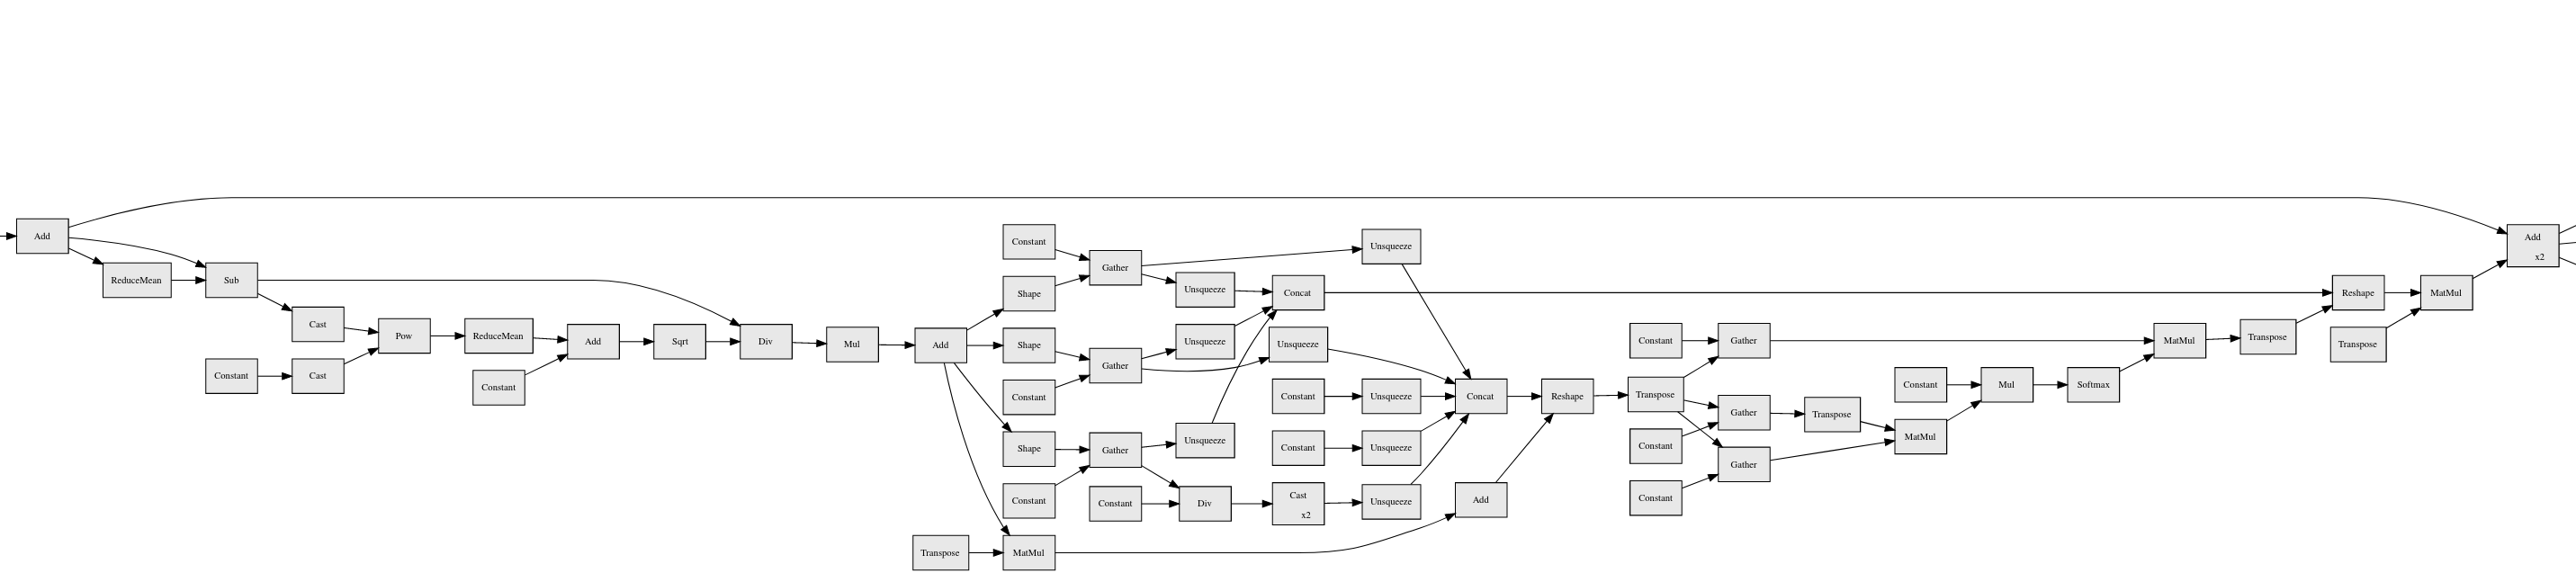
\includegraphics[width=1\textwidth,angle=90]{figures/research_methadology/model_overview.png}
    \caption{ConViT Layer}
    \label{fig:Convit_arch_}
\end{figure}


\newpage

\subsection{Grid Search Function}
\label{grid_search}

\begin{lstlisting}[language=Python, frame=single, label={lst:grid}, caption={Grid Search Hyper Parameters}]
def grid(self):
        para, parb, parc = (self.args[arg] for arg in args)
        search_space = [
        [para[idxa],parb[idxb],parc[idxc]] 
        for idxa in range(len(para)) 
        for idxb in range(len(parb))
        for idxc in range(len(parc))]
        return [' '.join([key+' '+str(arg) 
               for key, arg in zip(self.args,par_comb)]) 
               for par_comb in search_space]
\end{lstlisting}
\newpage
\subsection{Tilt and Shift Lense Example}
\label{sec:tilt shift}

\begin{figure}[ht!]
    \centering
    \specialrule{0.01em}{1em}{1em}
\begin{subfigure}[b]{0.5\textwidth}
    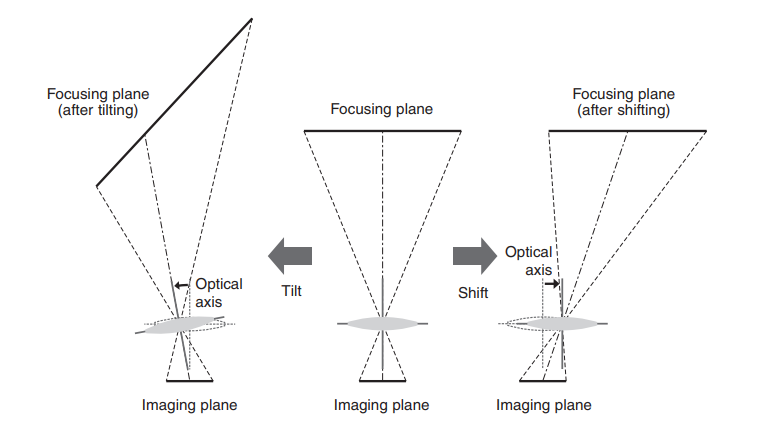
\includegraphics[width=\textwidth]{figures/appendix/tilt_shif_example.png}
    \label{tilt_diagram}
    \caption{Tilt Shift Optical Diagram}
\end{subfigure}
\hspace{5mm}
\begin{subfigure}[b]{0.5\textwidth}
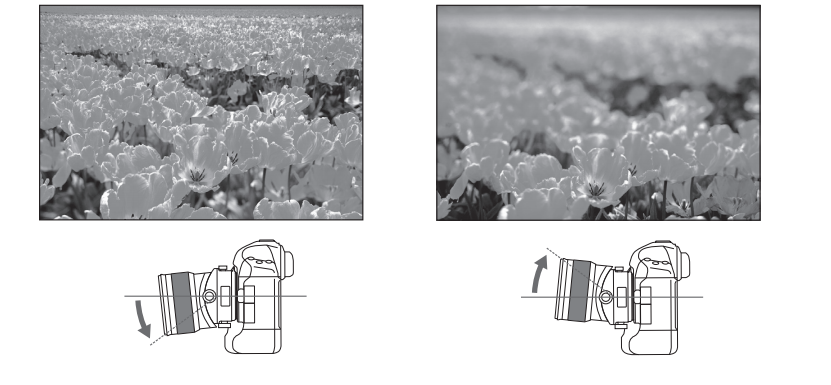
\includegraphics[width=\textwidth]{figures/appendix/tilteffect.png}
\label{tilt quality eg 1}
\caption{Tilt Shift Qualitative Example}
\end{subfigure}
\hspace{5mm}
\begin{subfigure}[b]{0.5\textwidth}
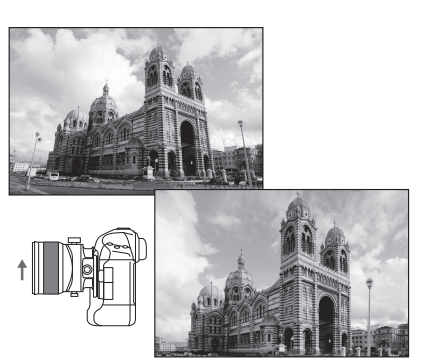
\includegraphics[width=\textwidth]{figures/appendix/shifteffect1.png}
\label{tile quality eg 2}
\caption{Tilt Shift Qualitative Example Architectural Photography Perspective Correction}
\end{subfigure}
    \caption{Tilt and Shift Example \cite{Cannon2019}}
    \label{fig:tilt shift all egs}
\specialrule{0.01em}{1em}{1em}
\end{figure}


\newpage

%%%%%%%%%%%%%%%%%%%%%%%%%%%%%%%%%%%%%%%%%%%%%%%%%%%%%%%%%%%%%%%%%%%%%%%%%%%%%%%%%%%%%%%%%%%%%%%
\subsection{Aesthetics with Attributes Database (AADB) }
\label{iaqa datsets appendix} 
This dataset was introduced by \cite{Kong2016}  and consists of 10k images. It is available online, however only with Mandarin file details. 

S. Kong et al.\citeaupurpose{Kong2016} purpose the datasets as a solution to some the pitfalls of other large-scale datasets, such as class imbalance and the inability to ascertain whether the same user has voted multiple times. AADB was produce by web-scraping from Flickr and random-sampling before abating ground truth from five different individual raters to then compile a confidence score for each attribute. 

The MOS scores are treated as a continuous variable rather than being thresholded into a good or bad category. 
\pagebreak 

\begin{figure}
\centering
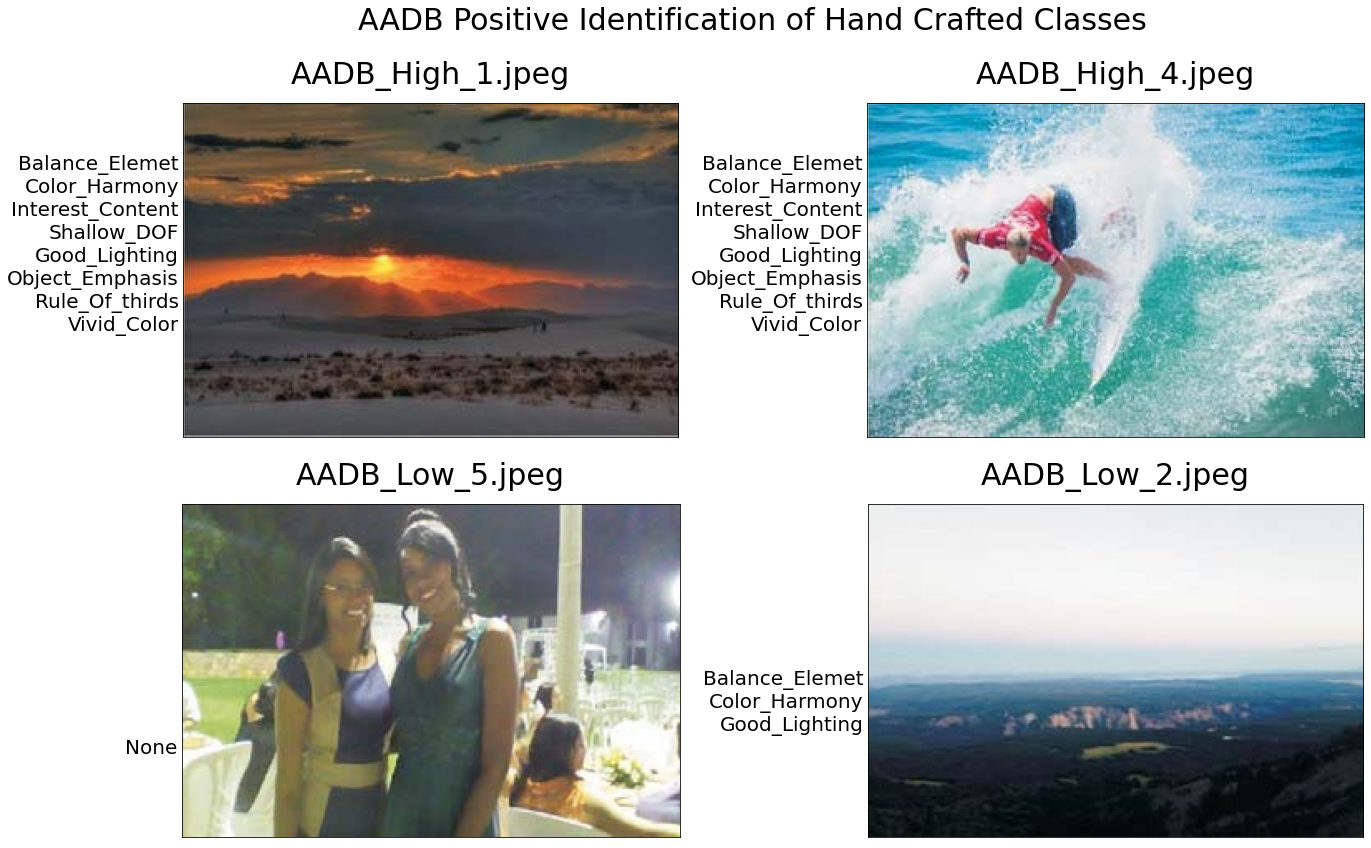
\includegraphics[width=0.9\textwidth]{figures/database_ims/AADB_2.png}
  \caption{\label{fig:AADB_1} AADB hand crafted classes}
  \label{fig:AADB1}
\end{figure}

\ref{fig:AADB_1} shows subjectively that those with a high number of aesthetic attributes are associated with binary classes of high and low aesthetic image quality. Top row images clearly showing high dynamic range, preservation of The dataset is split into high and low and author use. This in combination with aesthetic attributes for algorithmic inference of high or low images based on aesthetic attributes. 

\begin{figure}[hp]
\centering
 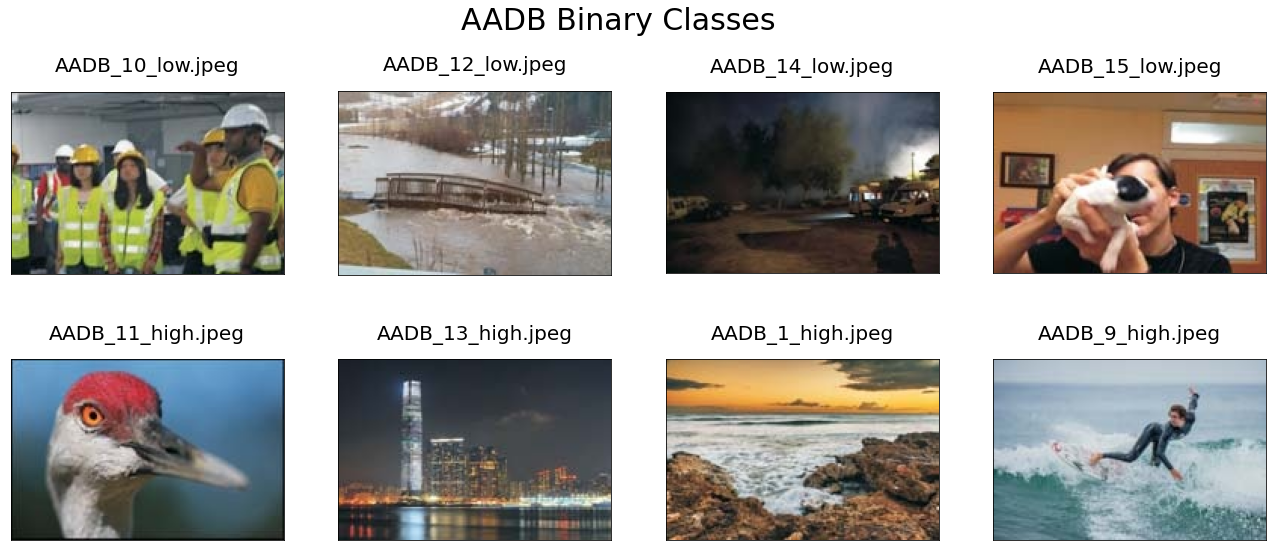
\includegraphics[width=0.9\textwidth]{figures/database_ims/AADB_1.png}
  \caption{\label{fig:AADB_3} Examples of AADB data-set binary classes}
  \label{fig:AADB3}
\end{figure}


\ref{fig:AADB_3} gives some insight into what high and low images 'look' like, and it is clear to the human/subjective eye that even from a small number of images that aspects such as multiple salient objects - where the foreground object is out of focus (top right) - are attributes of low quality images. 

However, this also highlights the high level of potential for ambiguity, wherein other images shallow DOF indicated by image features such a bokeh and high levels of blurriness around are also present in low quality images. Clear visual comparisons appear in figure \ref{fig:AADB_3} bottom left and AADB \ref{fig:AADB_3} top right, where both images have DOF - however, the bottom left high quality image has a salient object (bird) which is in focus where AADB 15 has a salient object (animal) out of focus. 

Ground truth within the dataset was provided by Amazon Mechanical Turk and images within this dataset have controls applied, such as the exclusion of synthetic or heavily edited images and images tagged with qualities \textit{interesting content, object emphasis, good lighting, colour harmony, vivid colour, shallow depth of field, motion blur, rule of thirds, balancing element, repetition,  symmetry}. These are showing in \ref{fig:AADB_3}, and also provide an insight into high and low quality images. 





%%%%%%%%%%%%%%%%%%%%%%%%%%%%%%%%%%%%%%%%%%%%%%%%%%%%%%%%%%%%%%%%%%%%%%%%%%%%%%%%%%%%%%%%%%%%%%%%%%%%%%%%%%%%%
\subsubsection{Aesthetic Rating Online Database AROD}


AROD was compiled from images from Flickr between January 2004 and November 2016\cite[3]{Schwarz2018a} and takes note of the number of 'faves' and 'likes' of the images. 

They propose a scoring function into high and low categories. This presents a very different distribution of images than is seen elsewhere, and while dataset size is significant, the criteria for scoring data remains somewhat distinct from others where thresholded from a normal distribution. 

The  ground truth of this dataset is taken from a much larger sample of raters, with an mean of 7k data-points per image. The authors make use of AMT to validate the usefulness of the derived ground truth metric that is computed from uncontrolled user clicks. 

The final model is then trained on ResNet50 and produces 75.83 accuracy - it is, however, unclear whether training a binary classifier in this way would perform well on a bench-marking dataset such as AVA, as the authors do not provide evaluation metrics on datasets used elsewhere.
 

\begin{figure}[htp]
\centering
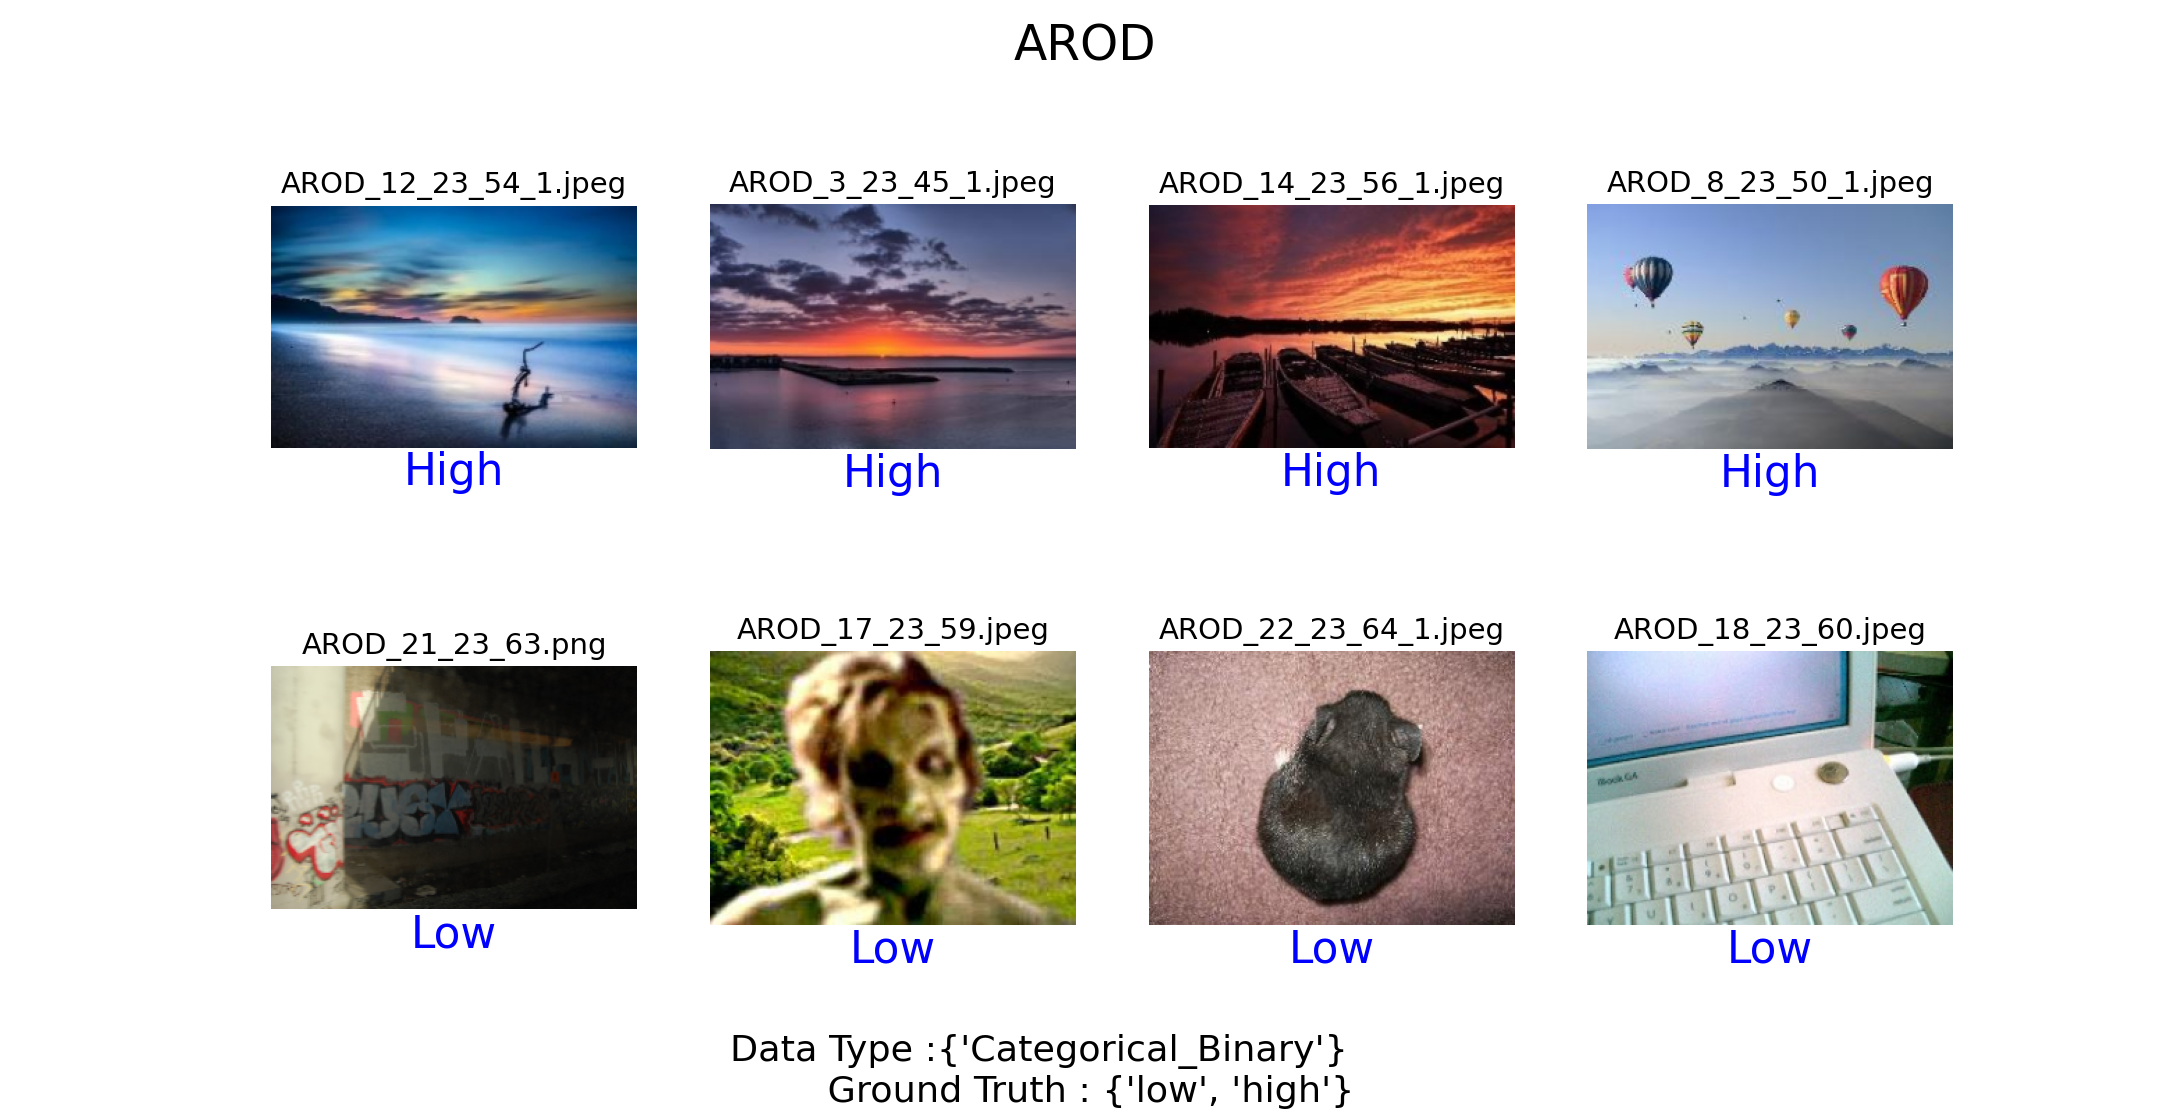
\includegraphics[width=0.9\textwidth]{figures/database_ims/AROD.png}
  \caption{\label{fig:AROD} AROD data-set binary classes top: high, bottom: low}
  \label{fig:AROD_}
\end{figure}

Note centre left, where the salient object is out of focus and the background is in focus in middle bottom left - this is subjectively apparent across datasets where, within a class, there are often images that apparently have otherwise similar visual appearance but where there remains a contradiction of an aesthetic principle (that the salient object should remain in focus).\\\


%%%%%%%%%%%%%%%%%%%%%%%%%%%%%%%%%%%%%%%%%%%%%%%%%%%%%%%%%%%%%%%%%%%%%%%%%%%%%%%%%%%%%%%%%%%%%%%%%%%%%%%%%%%%%
\subsection{ALIPR}


This dataset represents a unique example of sentiment tagged images. The 
authors also highlight the pitfalls of using crowd sourced MOS scores for sentiment; this dataset presents a novel approach for inferring individual image aesthetics to augment blunt MOS rated images. 

The dataset is compiled by \cite{Datta2008} and is and early example of an IAQA dataset. This was derived using \cite{Li2003} developed by \citeauthor{Wang2002} and is an example of building on existing hand-crafted feature work within IQA. 

It was part of hand-crafted feature selection for rating images based on 10 different emotions: \textit{Surprising, Amusing, Pleasing, Exiting, Adorable, Boring, Scary, Irritating, Other, No Feeling}. 


The authors aggregate data for descriptive purposes and employ traditional regression analysis rather than for machine learning on their relatively small dataset. The finding, while interesting, also highlights that many of the images either within the category of 'no feeling' were pleasing of boring. This highlights the ambiguity of assessing the sentiment of images.



\begin{figure}[hp]
\centering
 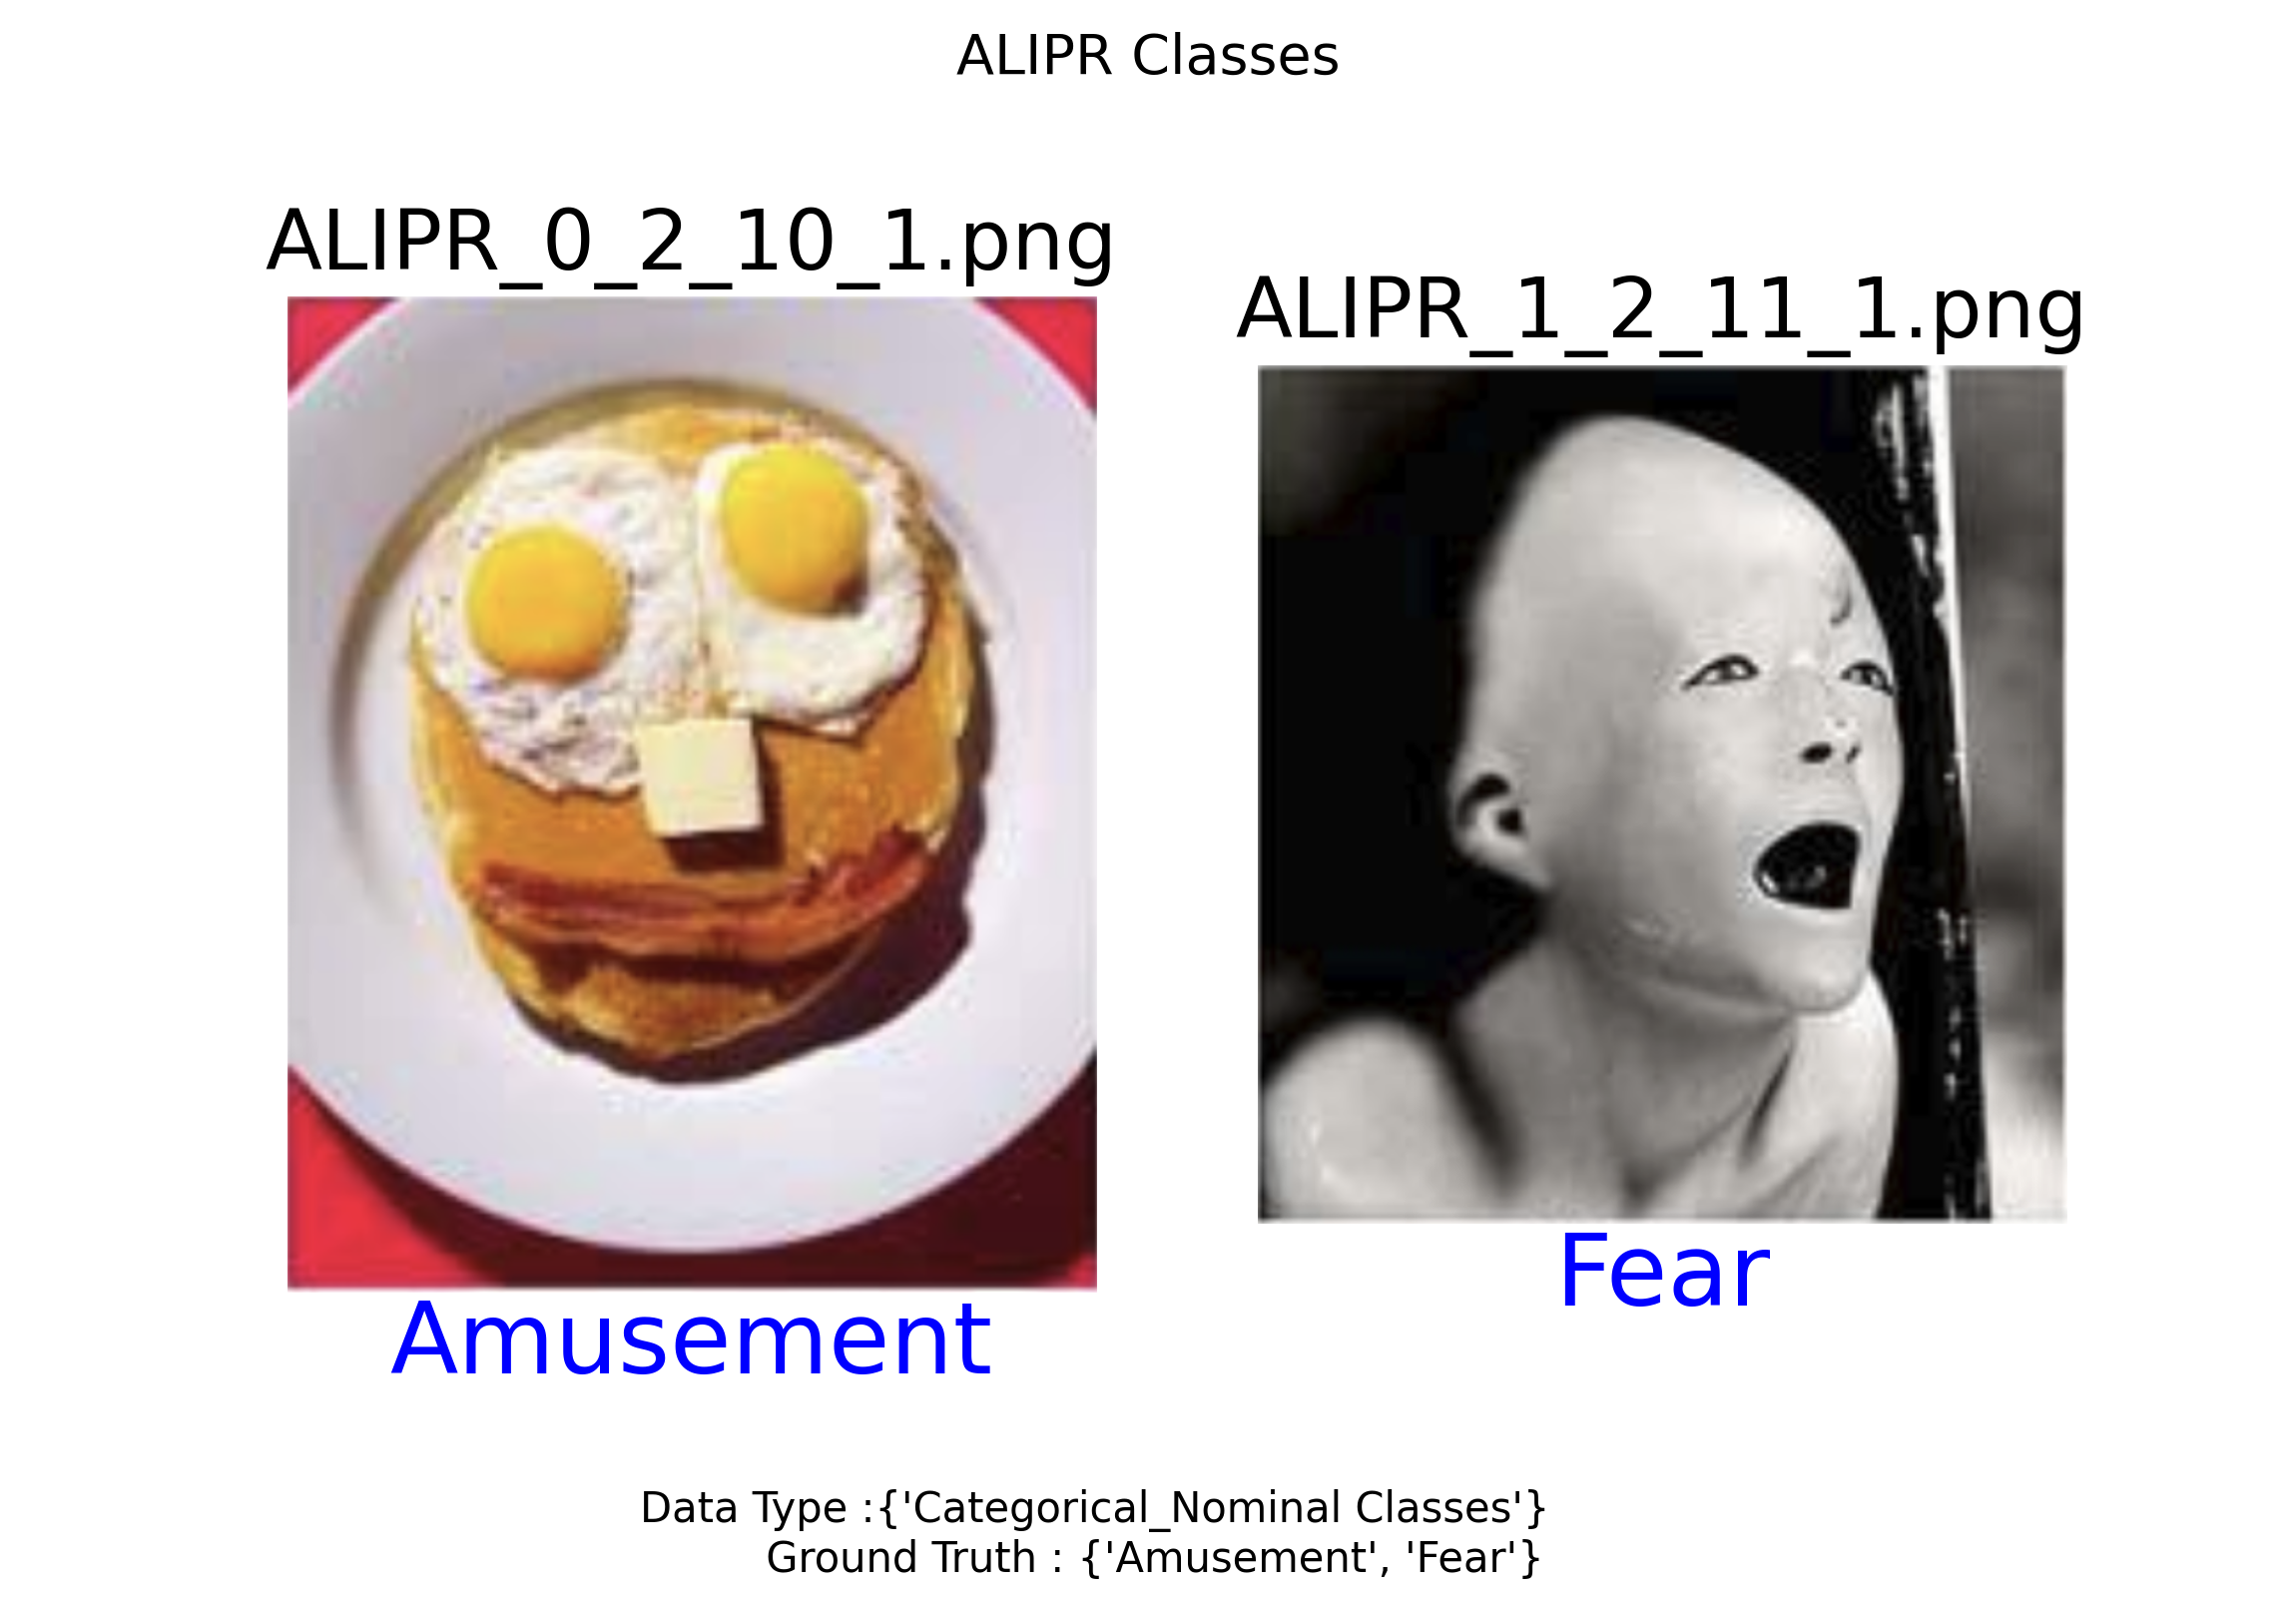
\includegraphics[width=0.6\textwidth]{figures/database_ims/ALIPR Classes.png}
 
  \caption{\label{fig:ALIPR} Examples of ALIPR nominal classes of sentiment tagged images}
  \label{fig:ALIPR_}
\end{figure}



%%%%%%%%%%%%%%%%%%%%%%%%%%%%%%%%%%%%%%%%%%%%%%%%%%%%%%%%%%%%%%%%%%%%%%%%%%%%%%%%%%%%%%%%%%%%%%%%%%%%%%%%%%%%%

\subsection{Aesthetic Visual Analysis AVA}

The AVA dataset that is the subject of this thesis is the third largest dataset reviewed within this section, and remains the most well established and canonised example of an IAQA. It is cited within 203 IEEE journals and 305 journals more widely \cite{AVA2012}. 

Further, it also maintains the most normal distribution, which is lower than that of other datasets such as PhotoNet. Further still, the distribution of the number of ratings is more approaching normal than the datasets of photo.net, which has large negative skew. 

The AVA\cite{Jin2016,Hosu2019,She_2021_CVPR,Lu2015a,Redi2015a,Chen2017,Cui2019,Simond2015,Kang2020,Yang2019,Li2020a, Jin2020, Wu2016,Sheng2018,Ma2017,Liu2017,Mavridaki2015, Aydin2015,Spathis2016} database is the database used within this study, and is to date the largest bench-marked dataset from a single source\cite{Hosu2019,She_2021_CVPR}. 

The AVA dataset was originally scraped from DP.Challenge.com (the namesake of the earlier database).  Each image within the AVA Dataset is ranked from 0-10  with (insert mean number of votes per image). 

The images are voted on by challenge participants, and voting can take place both during and after competitions.


%%%%%%%%%%%%%%%%%%%%%%%%%%%%%%%%%%%%%%%%%%%%%%%%%%%%%%%%%%%%%%%%%%%%%%%%%%%%%%%%%%%%%%%%%%%%%%%%%%%%%%%%%%%%%%%%%
\subsection{Chinese University of Honk - Kong-Photo Quality (CUHK-PQ)}

The CUHK-PQ dataset was introduced by\cite{Tang2013a} and consists of 17,673\cite{Tang2013a}  $\sim$ 17,613\cite{Murray2012} high quality images scraped from photo communities and low quality provided by university students with meta data on the score. The dataset also excludes photos with less than 100 votes to ensure a high degree of confidence. Further, the dataset consists of only absolute top and bottom quality classes {1 and 10} where voters on dp.challage.com are able to score images on a scale of 1-10. 

\begin{figure}[hp]
\centering
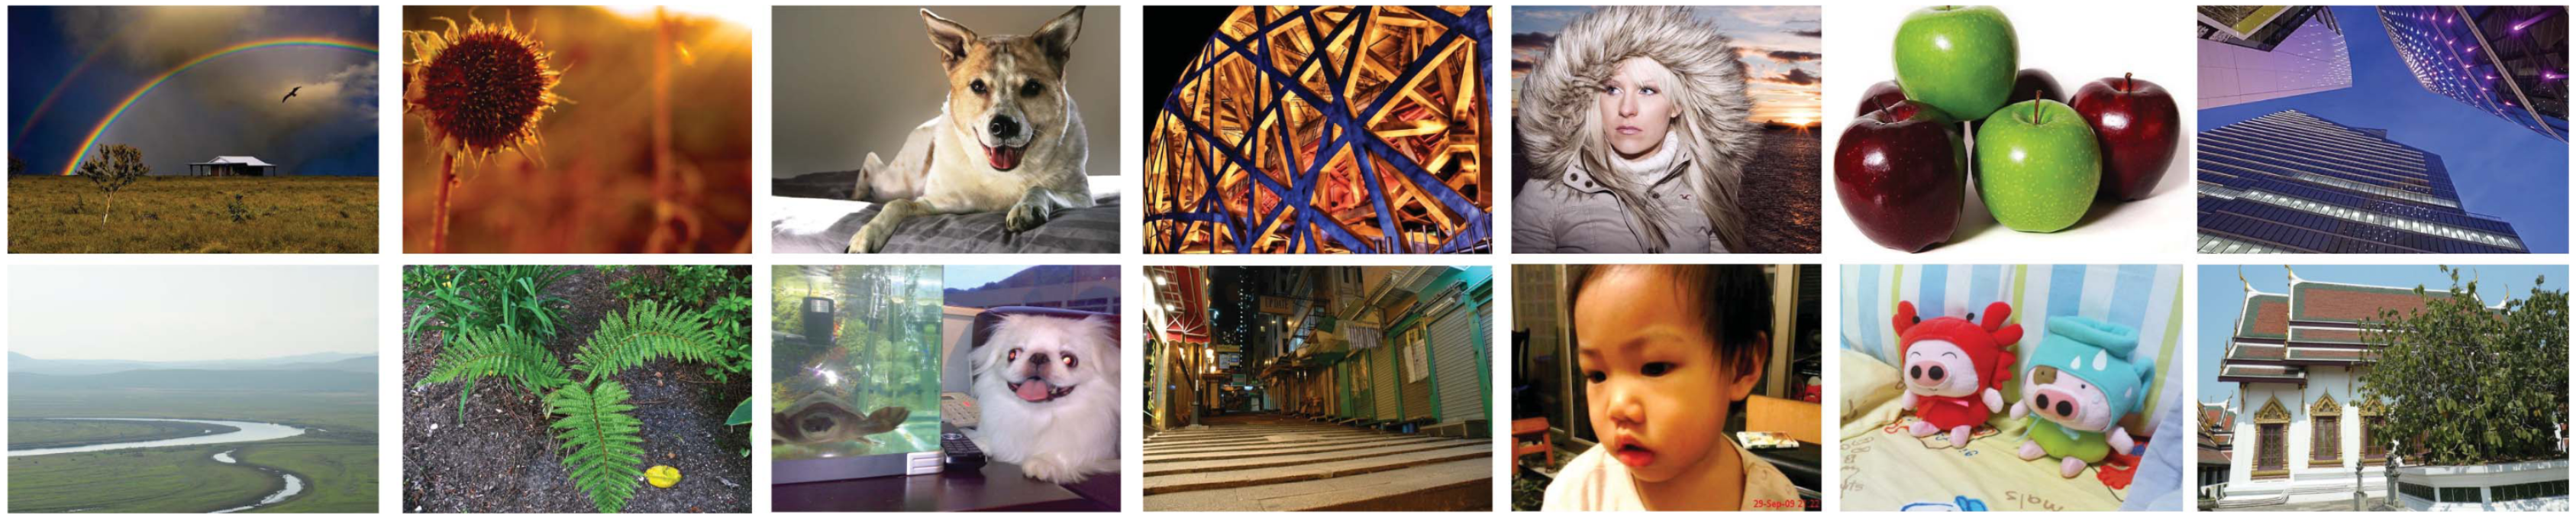
\includegraphics[width=0.9\textwidth]{figures/database_ims/CUHK-PQ_c.png}
  \caption{\label{fig:Data_CUHK} some examples of high and low quality images form the CUHK-PQ dataset - top is high and bottom is low quality}
  \label{fig:Data_CUHK_}
\end{figure}

The CUHK-PQ has a 0.5/0.5 test train split.  This dataset was compiled largely with an objective on undertaking machine learning with hand-crafted features. 

Others, such as \cite{Lo2013,Cui2019}, have used a subset of this dataset to perform IAQA experiments. Images are further sub-grouped into scene categories of: 
$$\in \{landscape, plant, animal, night, human, static, architecture \} $$

%%%%%%%%%%%%%%%%%%%%%%%%%%%%%%%%%%%%%%%%%%%%%%%%%%%%%%%%%%%%%%%%%%%%%%%%%%%%%%%%%%%%%%%%%%%%%%%%%%%%%%%%%%%%%
\subsection{DP Challenge}

\begin{figure}[hp]
\centering
 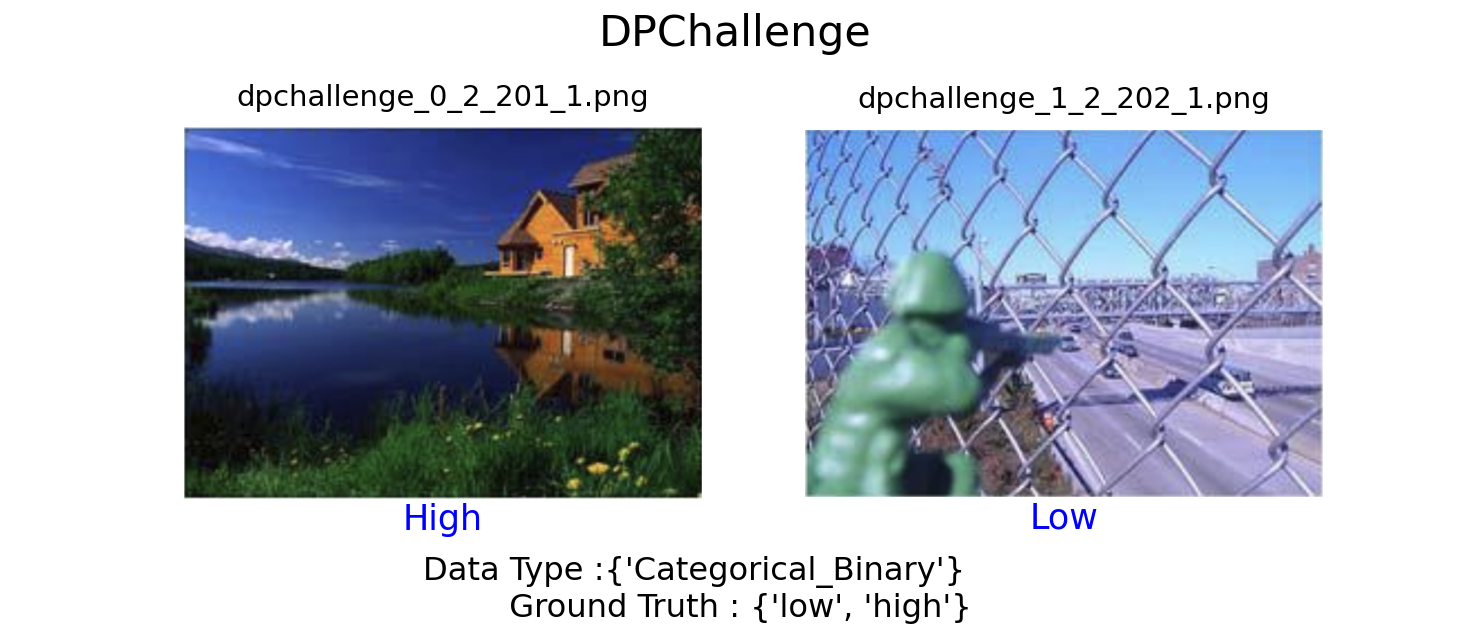
\includegraphics[width=0.6\textwidth]{figures/database_ims/DPChallenge.png}
  \caption{\label{fig:dpchall} DPChallange Dataset binary classes \textbf{left} high quality \textbf{right} low quality}
  \label{fig:dpchall}
\end{figure}


Were amongst the earliest examples of an IAQA dataset\cite{Yang2019} and present the first dataset that is thresholded into binary categories \textit{high} and \textit{low} categories\cite{Datta2008}. This dataset was initially defined in 2008, however has either been used or obtained new images by \cite{Jin2019,Dhar2011,Wu2011,Lou2008,Aydin2015,Gadde2011,Ke2006,Gao2015a,Nishiyama2011} and others. DP.challenge.com is also the source of the AVA bench-marking dataset \cite{Murray2012}.

To date, there are 330k images on the www.dpchallenge.com and it remains the largest source of images with recorded MOS that are freely available. 




%%%%%%%%%%%%%%%%%%%%%%%%%%%%%%%%%%%%%%%%%%%%%%%%%%%%%%%%%%%%%%%%%%%%%%%%%%%%%%%%%%%%%%%%%%%%%%%%%%%%%%%%%%%%%%%%%%%%

\subsubsection{Flickr AES}

The three datasets that are subsets of available images on the Flickr photo-sharing site are focused on particular fields of study, where researchers have required data on how individuals have related images. There are several so-called Flicker datasets, and the term has been somewhat ambiguously used within the literature. 

\cite{Yin2012} compile a dataset of 9,600 images with geotagging from Twitter, located from a large auxiliary dataset of 32,00 images. With 8 scene categories, where images are selected from top and bottom categories.

\cite{Ren2017} collected Amazon Mechanical Turk (AMT) ratings from 1-5 by five different workers to create ground truth. The 4,737 test images of  the dataset proposes the authors are also able to model how individual labels and measure against image datasets. 

\begin{figure}[hp]
\centering
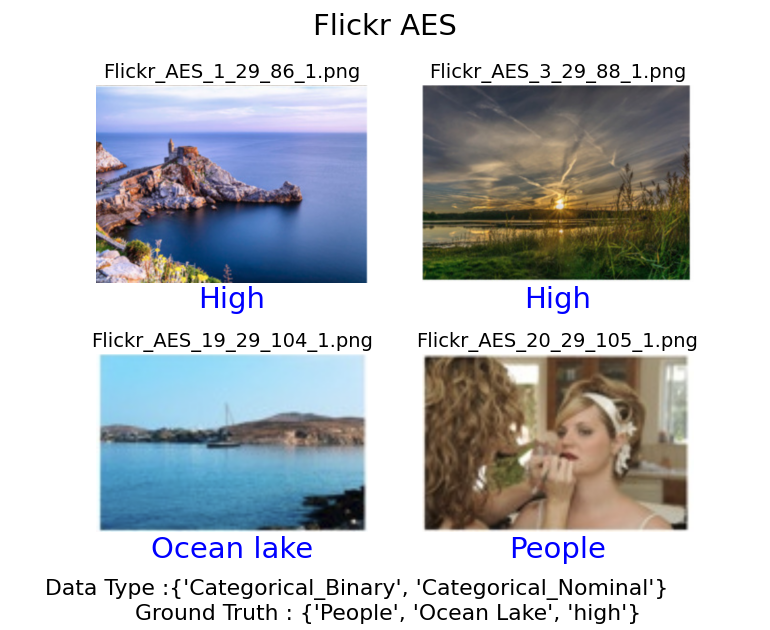
\includegraphics[width=0.6\textwidth]{figures/database_ims/Flickr AES.png}
  \caption{\label{fig:Flickr_AES} Examples of 7 AES data-set binary classes}
  \label{fig:AES_Example_}
\end{figure}

\cite{Chen2016} web scraped 70,00 $\sim$ 90,00 images from 35 identified Flickr groups. They treat each image set separately, and do not provide test training splits or public versions of the dataset. The largest early example of Flickr as a data source is \cite{Cheng2012}, who scraped 80,000 highly rated images for unsupervised learning using hand-crafted features. 

\cite{Schifanella2015} also compile their own dataset from Flickr to highlight challenges in deriving user produced data from social media sources (such as Flickr) where the number of  likes is taken as a proxy for quality.

\pagebreak




%%%%%%%%%%%%%%%%%%%%%%%%%%%%%%%%%%%%%%%%%%%%%%%%%%%%%%%%%%%%%%%%%%%%%%%%%%%%%%%%%%%%%%%%%%%%%%%%%%%%%%%%%%%%%%

\subsubsection{Image Aesthetic Database(IAD)}

To date, this is the largest dataset of IAQA and is derived from DPChallenge (300k) images and w.2 million images form PhotoNet. The mean score image from PhotoNet\cite[12]{Lu2015a} thresholded images from dpchallenge.com and PHOTO.NET. 

The threshold boundary for PHOTO.NET is 4.88 and they remove all data within the AVA dataset inter quarterly range (IQR), and are left with only the top and bottom 20\% of images.  \ref{fig:IAD} shows examples of high and low quality images after thresholding. 

\begin{figure}[hp]
\centering
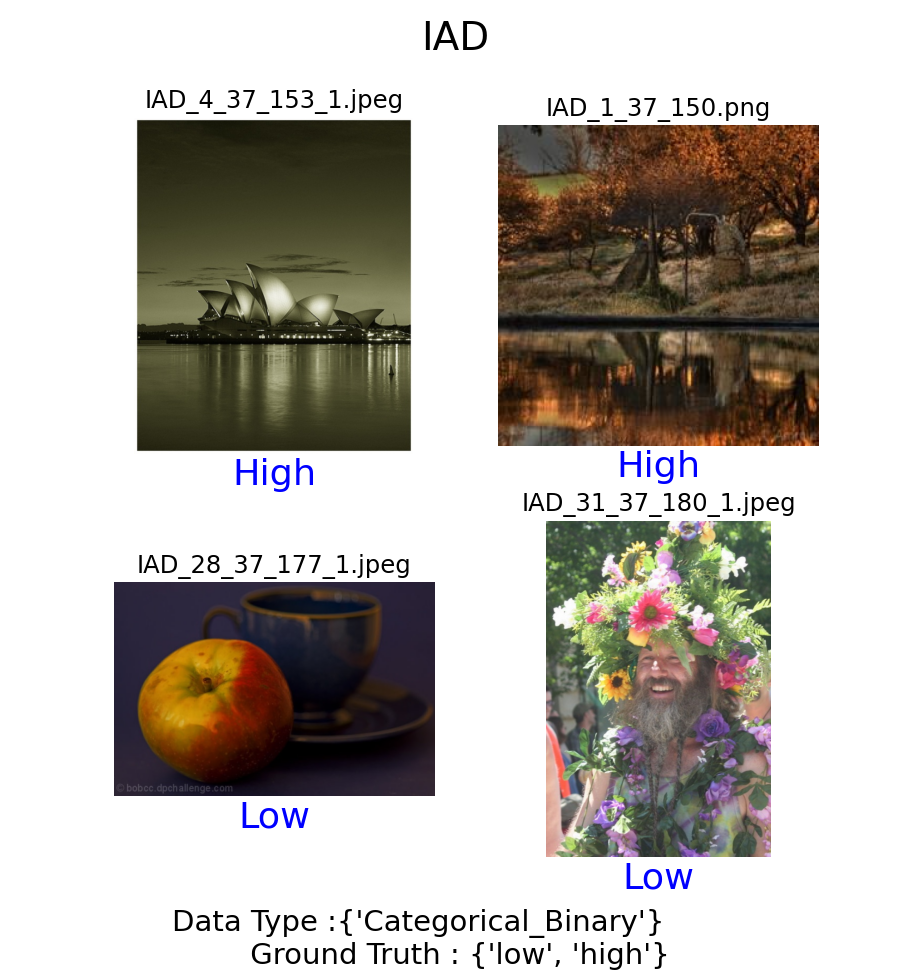
\includegraphics[width=0.6\textwidth]{figures/database_ims/IAD.png}
  \caption{\label{fig:IAD} Examples of IAD data-set binary classes}
\end{figure}
DP.challenge.com has a rating of 1-7 compared to AVA's 1-10, and their whole threshold follows on in principle. Similarly, the distribution of photo.net surfers  - for being more atypical to DPChallenge images (this in itself is an interesting and noteworthy phenomenon) and in spite of a much high number of images, show distribution of scores less uniform and with a much higher degree of variability.

while \citeauthor{Lu2014a}\cite{Lu2014a} were able to leverage an increased dataset size for state of the art results at the time of publication, it is noteworthy that many more recent publications have far surpassed their accuracy using only the AVA bench-marking dataset \cite{Zhang2021d,Ma2017,She_2021_CVPR,Kong2016,Jin2016}. 

Further, the authors make mention of 300k images from DPchallenge; to date, there are 330k images and the date they were rescraped would have therefore included the AVA test images, given that it would not have been possible to obtain 300k images from Dpchallenge in 2016 without including the $\approx$ 20k test images (as there would not have been 90k 'new images' without including them).  

%%%%%%%%%%%%%%%%%%%%%%%%%%%%%%%%%%%%%%%%%%%%%%%%%%%%%%%%%%%%%%%%%%%%%%%%%%%%%%%%%%%%%%%%%%%%%%%%%%%%%%%%%%%%%%%%

\subsubsection{Photo Critique Captioning Dataset PCCD}

This dataset consists of images scraped from a single source \cite{Chang2017,guru} and is based on professionally reviewed of photos where comments are given on general impression, composition,  perspective, colour and lighting with a subset of photo, DOF, use of camera exposure and shutter-speed. 

Figure \ref{fig:PCCD} shows some particularly high quality images subjectively.
\begin{figure}[hp]
\centering
 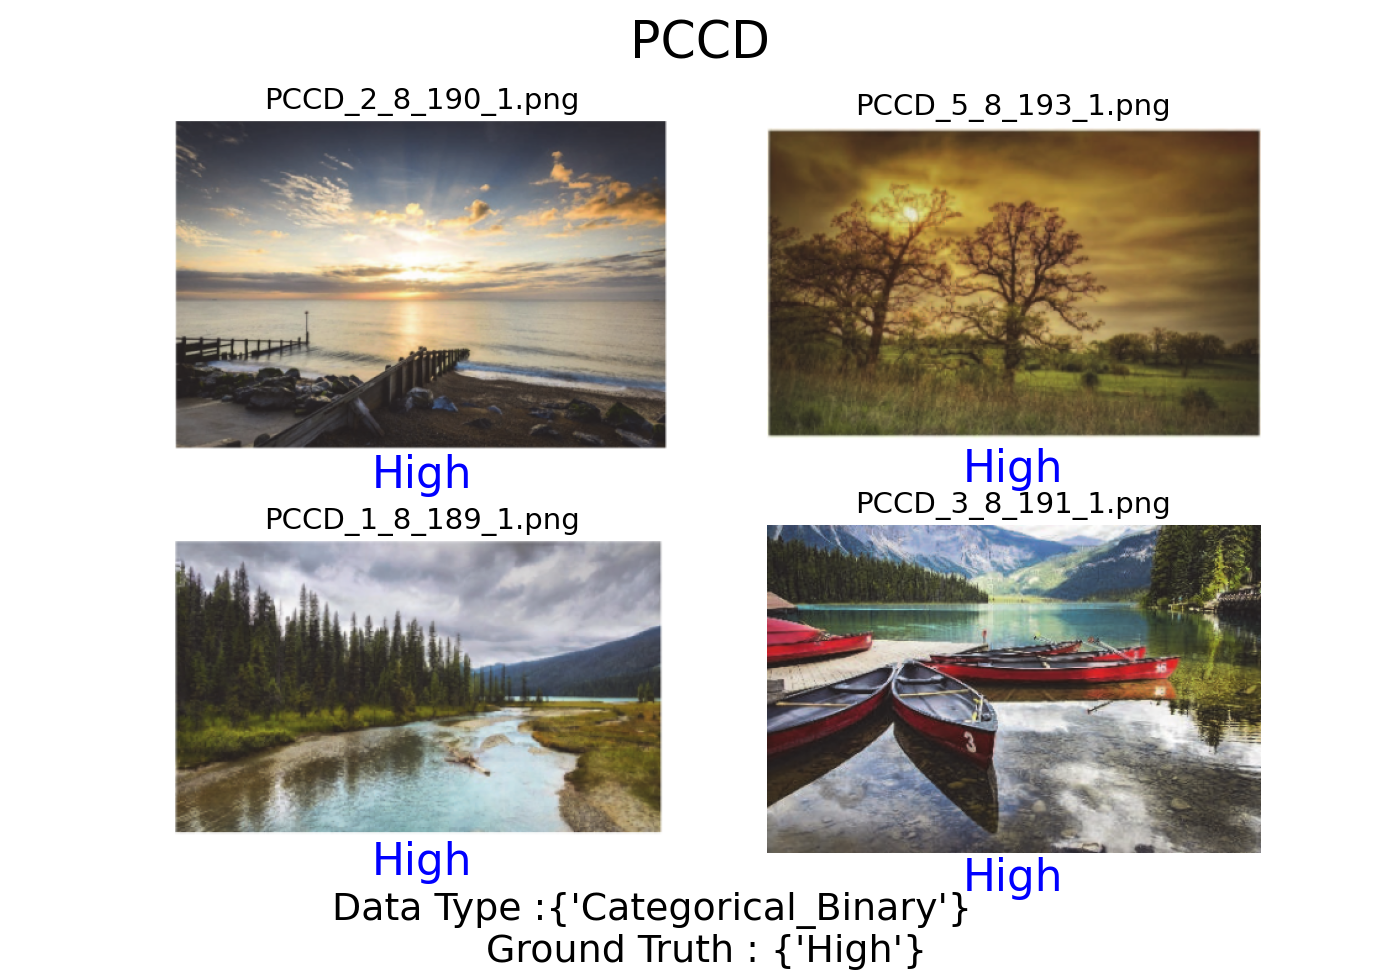
\includegraphics[width=0.6\textwidth]{figures/database_ims/PCCD.png}
  \caption{\label{fig:PCCD} Examples of PCCD dataset}
  \label{fig:PCCD_}
\end{figure}

 One notable feature of this is the high ratio of comments to image, with $\approx$ 60k captions. Each image is given a numerical rating of 1-10. 
%%%%%%%%%%%%%%%%%%%%%%%%%%%%%%%%%%%%%%%%%%%%%%%%%%%%%%%%%%%%%%%%%%%%%%%%%%%%%%%%%%%%%%%%%%%%%%%%%%%%%%%%%%%%%%%%%%

\subsubsection{Photo.Net}


This originally consisted of 3,581\cite{Datta2006}  images, however later publications \cite{Joshi2011} augment this or re-scrape images to derive datasets of 20276  net. One distinction is that while many of the datasets are, in practice, thresholded into binary $\in \{good,bad\}$ that Photo.Net has ranked 1-7.

\begin{figure}[hp]
\centering
 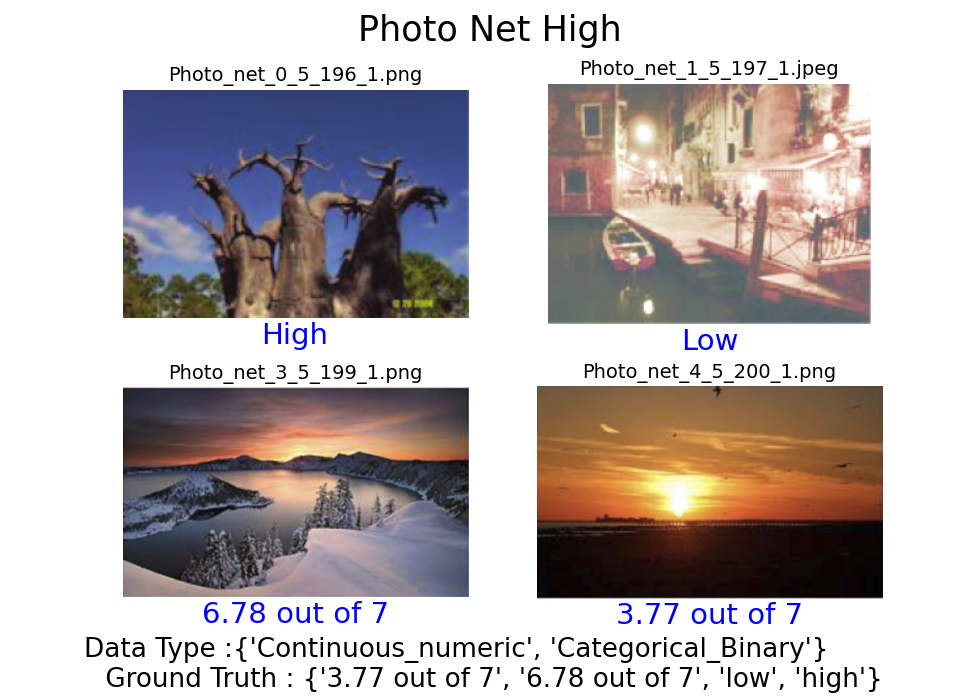
\includegraphics[width=0.6\textwidth]{figures/database_ims/Photo Net High.png}
  \caption{\label{fig:Pnet} Examples of PHOTO.NET}
  \label{fig:Pnet_}

\end{figure}





\subsubsection{Waterloo IAA}


This small dataset was compiled for content subjective assessment, while it is not in itself large enough to meaningfully conduct deep learning based approaches. 

\cite{Liu2017} compile a rich database of aesthetic features that are collated under controlled conditions. The associate publication also demonstrates, for instance, that it is difficult for humans to assess aesthetics from a single factor, but rather that it is in consideration of combinations of factors. 

The data was compiled using a computer program where users have a sliding scale, and are able to use a graphics user interface (GUI) in order to capture rating feedback from experimental subjects. The feedback is then used to subset the data for traditional statistical analysis, rather than machine or statistical learning. 

This represent a similar approach to AADB datasets in its rigorously paired down subcategories.  

\begin{figure}[hp]
\centering
 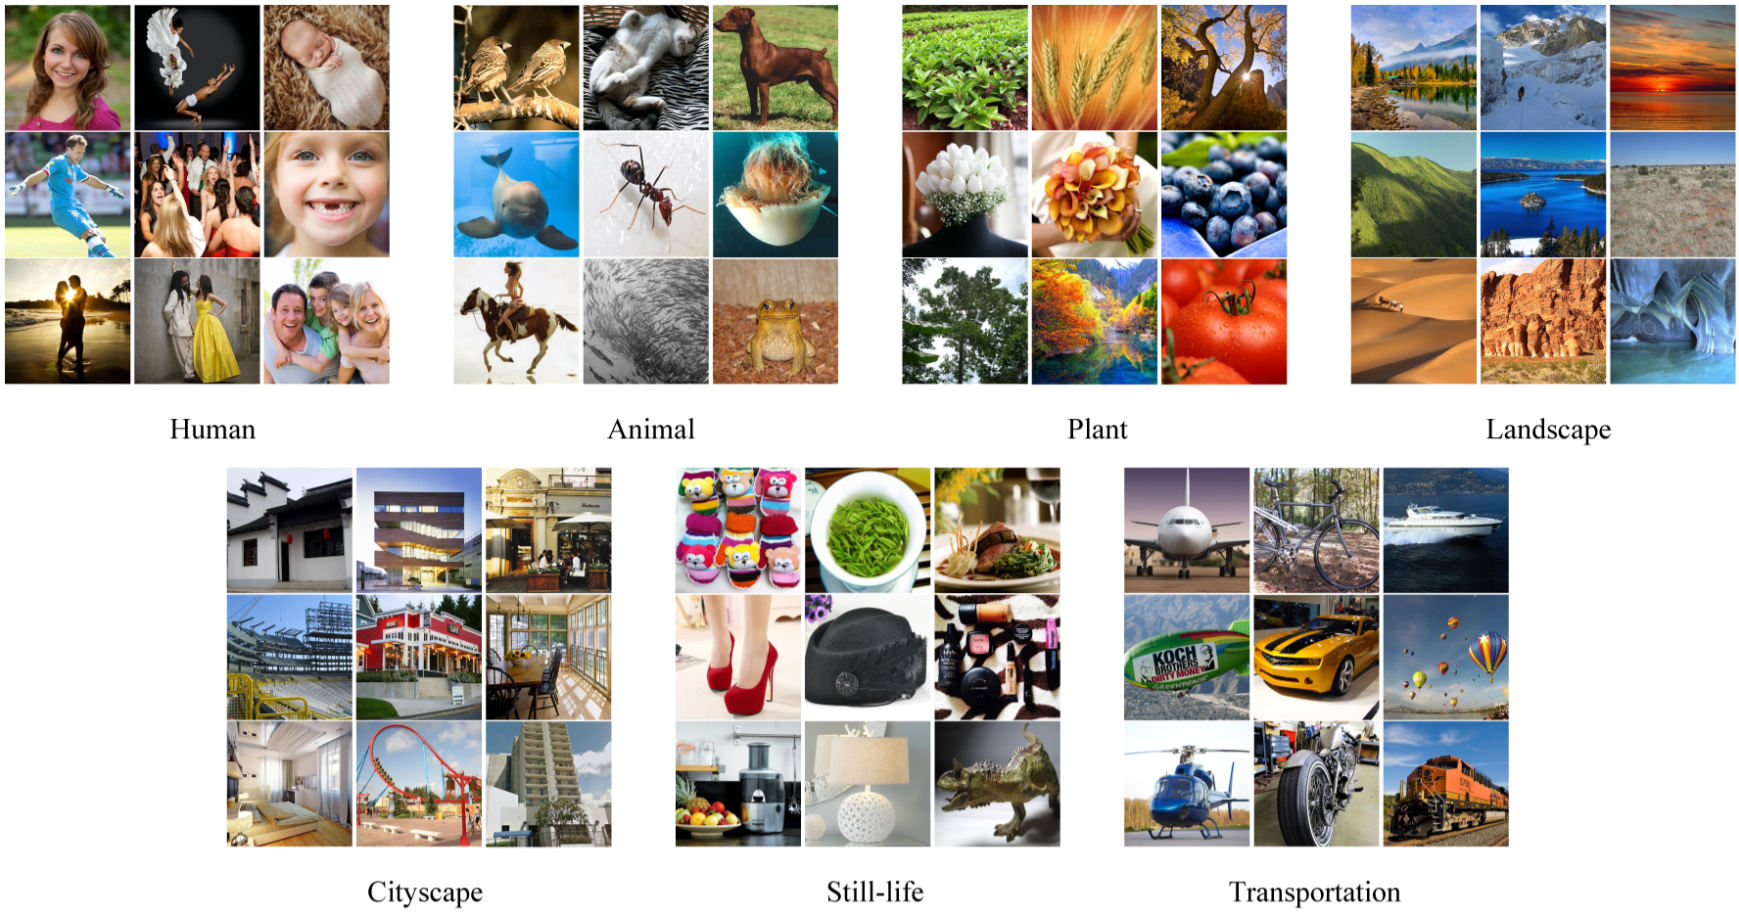
\includegraphics[width=0.9\textwidth]{figures/database_ims/WATERloo.png}
  \caption{\label{fig:Pnet} Waterloo class examples}
  \label{fig:Pnet_}
\end{figure}

Liu W.\cite{Liu2017} also apply high levels of scientific rigour to controlling the environment in which the data is captured from subjects, for example calibrating the screen and reporting its results. 


\subsection{Dataset Conclusion}

The datasets reviewed here are by no means exhaustive, and the review of IAQA datasets could comprise an entire literature review or survey paper in its own right. 

There are fascinating and bespoke examples of user rated databases and retrieval system such as Terra Galleria\cite{Quand-T} which are well canonised\cite{Mayssara2014, Hutchison2013, Joshi2011} images of a single genre, a single photographer, but with voting data of scores between 1-10. 

In addition to deep learning that has been leveraged for evaluation of individual artists such as Andy Lomas\cite{McCormack2021}, both of which are well canonised examples of more bespoke datasets. Some earlier examples of hand-crafted features scrape inames for a single source such as \cite{Cheng2012}. 

There are also dasasets on the wider domain of IAQA, such as Chinese Handwriting Aesthetic Evaluation Database CHAED \cite{Sun2015}.  

The terminology used, including abbreviations of different databases, are not consistent throughout the literature. This is for three reasons:

\begin{enumerate} 

\item First, that the source of the databases such as Flickr, DPChallange, or Photo.Net have been used within database nomenclature to indicate datasets, many of which are themselves subsets of other datasets, \cite{Spathis2016} also use the title of a paper as the acronym for a dataset that was created by the authors. 

\item Second, and perhaps tangential to the slippage in nomenclature between dataset and source, there there are some inconsistencies in literature for instance \cite{Kanwal2021} use the term Photo web citing \cite{Datta2006} where the term Photo.Net is used.

\item Third, that subsetting of datasets within individual publications, while retaining the super set name, makes the process of effective bench-marking and maintaining the official test train split. 
\end{enumerate} 

This is challenging, as it leads to potential for inconsistent benchmarking and may serve to dilute the absolute value of results where one subset may be present in test sets of another set with no clear way to ensure that there is not what is in effect a data leak by proxy, with \cite{Lu2015a} as an example of this.  

Further, and perhaps in support of evidence of some lack of cohesion within IAQA community, datasets are not always consistently cited for instance \cite[539]{Lo2013} cites \cite{Tang2013a} as a source dataset and then subset this into an new dataset with a different ratio of positive to negative class, which is then cited by \cite[4]{Kanwal2021} as Photo Databse. 

This is further compounded by the variability in nomenclature of derivative data sources such as dp.challenge and Flickr. (Further, the dataset size is not always consistently reported for individual dataset.) 

One aspect of useful further research would be to provide a consistent high level framework for IAQA dataset and a data schema, which might include a process of using image retrieval to check for duplication's and use of original site image ID's where for instance image ID's are used within image urls . 

An aspect of additional complexity is that there exists a high degree of sub-setting or creating new datasets, as can be seen in some of the more recent and smaller datasets. For instance, \cite{Jin2019} upscales the approach of \cite{Chang2017} onto an augmented AVA dataset by web scraping further images for dp.challenge.com. 


